\documentclass[times,11pt]{report}
\usepackage{fullpage}
\usepackage{graphicx}
\usepackage[colorlinks=true,linkcolor=black]{hyperref}
\usepackage{hyperref}
\usepackage{mathptmx} % - sets \rmdefault to 'ptm', i.e. times
\renewcommand{\familydefault}{ptm} % using \rmdefault here doesn't work
\begin{document}
\title{Savant Genome Browser: User Manual}
%\author{Marc Fiume \& Eric Smith}
\maketitle

\setlength{\parindent}{0pt} 
\setlength{\parskip}{2ex}

Authors: Marc Fiume \& Eric Smith\\
Contact: savant@cs.toronto.edu \\
Website: http://savantbrowser.com \\
\\
This document applies to Savant version 2.0.0\\

\newpage

\tableofcontents
\listoftables
\listoffigures

\newpage

\chapter{Introduction}

\section{What is Savant?}

Savant stands for ``Sequence Annotation Visualisation and Analysis Tool''. In other words, Savant is a program for visualising and analysing genomics data. It was designed to run quickly and efficiently on conventional desktop or laptop computers.

\section{Who Should Use Savant?}

Savant makes visualisation and analysis of genomics data very efficient. If you use genome browsers like UCSC or IGV or if you are a biologist or bioinformatician who works with genomics data, you should try Savant. 

\section{Getting Started}
Savant is designed to run on any operating system which supports Java Standard Edition 1.6 or 1.7.  In practice, it has been tested on Windows (XP, Vista, and 7; 32-bit and 64-bit), Mac OSX (10.6 and 10.7), and Linux (32-bit and 64-bit).  An internet connection is strongly recommended.

When you launch Savant, you will be presented with the start screen, which shows a list of recent projects and a feed of news stories from the Savant web-site.  If this is the first time you have launched Savant, there will be no recent projects, so the first thing you should do is choose \textit{File~\textgreater~Load~Genome} to tell Savant what reference genome you wish to work with.

\chapter{Projects and Tracks}

When working with Savant you will typically be working with a number of ``tracks'' which are organised together into a ``project''.  In addition to the tracks, a project file also maintains associated information, such as the reference genome, your browsing location, and any saved bookmarks. Each track normally corresponds to single data file, although there are exceptions (e.g. a BAM alignment track may also be accompanied by a TDF file containing coverage information to be displayed at lower resolutions).  In order to be loaded as a track by Savant, a file must be in one of the formats described in Table~\ref{NativeFileFormats}.  Files which are not already in one of those formats can be converted as described in \S\ref{UsingFormatDialog}.

\section{Projects}
Projects have a file extension of \textit{.svp}, and are typically stored in the \textit{.savant/projects directory}.  The project stores the following information:
\begin{itemize}
\item Reference genome
\item Absolute paths of all loaded tracks.
\item Current display mode of all tracks
\item Bookmarks
\item For variant data, a summary of which participants are controls or cases (see Chapter~\ref{Variants})
\end{itemize}


\section{Genomes}
Before loading any tracks, the project's reference genome must be established using the \textit{File~\textgreater~Load~Genome} command.  This genome is used to specify the lengths and names of all chromosomes or contigs in the data set; no other tracks can be loaded until the genome has been set.  In many cases, the genome will itself be a sequence track, which can be loaded from a file, from a URL, or from a remote data-source.

For the convenience of users, a variety of standard published genomes are available through the \textit{Load Genome} dialog.  The commonly-used genomes include a full sequence track along with associated tracks such as UCSC and RefSeq genes.  Less popular genomes may provide only a list of the chromosome names and their sizes.  The exact list is subject to change, and we welcome requests to add your favourite genomes to Savant's standard set.

In some unusual cases, you may wish to run Savant without any existing genome information.  In such cases, you can use the Load Genome dialog to specify a reference name and length.

\section{Tracks}

A track is an individual data set, usually corresponding to a single data file.  In a few situations a track may draw data from multiple data sources; this is the case for BAM alignment tracks which can have an associated TDF file containing coverage information to be displayed at lower resolutions.  In order to be loaded as a track by Savant, a file must be in one of the formats described in Table~\ref{NativeFileFormats}.  Files which are not already in one of those formats can be converted as described in \S\ref{UsingFormatDialog}.  If you attempt to load a track from one of the compatible file-types described in \S\ref{CompatibleFileFormats}, Savant will offer to format it first.

\subsection{Display Modes}
Every track type has one or more display modes.  Each of these modes is intended to emphasise a different aspect of the data. For instance, the \textit{Mismatch} mode for read alignment tracks, uses colours to emphasise mismatches in reads.  In contrast, the \textit{Read Pair (Arc)} mode emphasises the insert lengths, showing arcs between the mapped locations of paired reads, with the height of each arc proportional to the inferred insert size.  The display modes available for each type of track are described in \S\ref{TrackTypes}.

\subsection{Loading a Track}

A track is loaded by choosing one of the \textit{File~\textgreater~Load~Track} menu-items.  Track data can come from any of three different sources:  a local file, a URL, or an external data source.  \textit{Load Track from File} will present a file-chooser to let you select a local file.  \textit{Load Track from URL} presents a dialog which lets you type in an ftp://, http://, or https:// URL to be opened.

The \textit{Load Track from Other Datasource} menu-item presents the Savant repository browser, which lets you select one of the tracks which is available from savantbrowser.com.  In addition, this menu-item is also used by plugins such as the SQL and UCSC plugins to allow you to open a track using that plugin.

\subsection{Track Types}
\label{TrackTypes}

Savant supports five different types of tracks, which are described below.  Each track appears in a separate window, which can be manipulated as described in \S\ref{DockingFramework}.

At the right of the track is a legend which describes its contents.  Above the legend is a track-specific menu-bar which allows you to control the display and behaviour of that track.  This menu-bar will have at least two items:  Tools and Appearance.  In addition, some tracks have menu items which let you control \textit{Display Mode} and \textit{Interval Height}.

The \textit{Tools} menu provides useful functionality such as the ability to Lock a track (see \S\ref{TrackLocking}) and to copy the track's URL to the clipboard.  Track types which have the ability to filter their contents add a \textit{Filter\ldots} item to the Tools menu, which invokes a dialog to specify filter parameters.

The Appearance menu controls the track's colour settings.  For tracks which have a vertical scale (all but sequence tracks), the \textit{Scale to Fit} menu-item controls whether the track scales its y-axis to fit the size of the window or uses a vertical scrollbar when necessary.

\subsubsection{Sequence Tracks}
Sequence tracks take their data from a .fa or .fa.savant\footnote{.fa.savant files store sequence data in a format specific to Savant versions prior to 2.0.0.} file.  They display a sequence of colour-coded nucleotides.

Sequence tracks are often used by \textit{File~\textgreater~Load~Genome} to provide the reference genome for a project.  If you have more than one sequence track open in a project, you can use a sequence track's \textit{Tools~\textgreater~Set~as~Genome} menu-item to make it the reference genome.

\subsubsection{Interval Tracks}
Interval tracks display data from a Tabix file.  This is the track-type for genes and other interval-oriented data.

Interval tracks have two display modes:  Standard and Squish.  In Standard mode intervals are packed neatly so that none overlap; in Squish mode, the intervals are squished together on a single line.  These correspond to the Pack and Squish modes of the UCSC browser. 

In addition, interval tracks also have a number of Appearance options.  The \textit{Enable ItemRGB} option colours records based on the value of their ItemRGB column (for BED files which have that column).  Similarly, for BED files with a Score column, the \textit{Enable Score} option allows you to draw records with a transparency based on the Score value. The \textit{Display Alternate Name} option allows you to control which labels are displayed for the features (e.g. for gene tracks which may identify genes with both accession numbers and protein IDs).

\subsubsection{Alignment Tracks}

Alignment tracks display data from a BAM file.  They present reads in a choice of seven different display modes, listed in Table~\ref{AlignmentModes}.

\begin{table}[h]
\begin{center}
\begin{tabular}{|l p{12.5cm}|}
\hline
Standard & Displays the reads stacked vertically in the most efficient manner.  Colour indicates strand direction.\\
Mismatch & Like Standard, but also displays SNPs and indels.  Requires that the reference genome be an actual sequence track.\\
Read Sequence & Displays the reads stacked vertically, but colour indicates nucleotides.\\
Read Pair (Standard) & Reads are stacked vertically, with paired reads at the same altitude.\\
Read Pair (Arc) & Read pairs are shown using arcs, where the height of the arc corresponds to the inferred insert size.\\
SNP & For each location, all the base-reads supporting a particular call are stacked vertically.  This is intended to make SNPs more prominent.\\
Strand SNP & Like SNP mode, but reads from the forward and reverse strands are grouped separately.\\
\hline
\end{tabular}
\end{center}
\label{AlignmentModes}
\caption{Alignment Track Display Modes}
\end{table}

In addition to the display mode, you can also adjust the appearance of the Standard, Mismatch, and Read Sequence modes by using the \textit{Enable Base Quality} and \textit{Enable Mapping Quality} items from the \textit{Appearance} menu.

When the visible range is large enough that individual reads would not be visible, Savant will display a coverage graph (\S{GeneratingCoverageFiles}) in place of the normal display.

\subsubsection{Continuous Tracks}
Continuous tracks display continuous-valued data from TDF or BigWig files.

\subsubsection{Variant Tracks}
Variant tracks display structural variation data from Tabix-formatted VCF files.  The vertical axis is used to indicate the individuals whose data makes up the file.  Data from all loaded variant tracks is aggregated in the Variation sheet described in \S\ref{Variants}.

\chapter{Formatting and Loading Data}

\section{Supported File Formats}

Savant natively supports a number of standard file formats which are indexed to ensure speedy data retrieval.  In addition, Savant has the ability to reformat several other common formats in order to make them usable by the program.

\subsection{Native File Formats}

Savant natively supports the following standard file formats.  These are formats which Savant can read directly with no extra processing.  In most cases, these files consist of a main file which contains the actual data and an index file which must be present in the same location as the data file in order to provide fast random access to that data.

\begin{table}[ht] 
\begin{center}
\begin{tabular}{|l|l|l|l|}  
\hline                      
Format & Description & Data File & Index File\\
\hline                    
\href{http://genome.ucsc.edu/goldenPath/help/bam.html}{BAM} & Nucleotide  sequence alignments & .bam & .bai \\
\href{http://genome.ucsc.edu/goldenPath/help/bigWig.html}{BigWig} & Continuous-valued data & .bw & \\
\href{http://genetics.bwh.harvard.edu/pph/FASTA.html}{FASTA} & Nucleotide sequences & .fa & .fai \\
\href{http://samtools.sourceforge.net/tabix.shtml}{Tabix} & Genes, intervals, variants, and other localised data & .gz & .tbi \\
\href{http://www.broadinstitute.org/igv/TDF}{TDF} & Any continuous-valued data & .tdf & \\
\hline     
\end{tabular} 
\caption{Native File Formats}
\label{NativeFileFormats}
\end{center}
\end{table} 

\subsection{Compatible File Formats}
\label{CompatibleFileFormats}

These are formats which Savant can convert into one of its native formats.  When using a file in one of these formats, it must first be converted into one of Savant�s native formats.
You can convert these files either by using choosing Format from Savant�s File menu, or by using Savant�s \textit{FormatTool} utility.

\begin{table}[ht] 
\label{CompatibleFileFormatsTable}
\begin{center}
\begin{tabular}{|l|p{7.5cm}|l|}  
\hline                      
Format & Description & Converted To\\
\hline                    
\href{http://genome.ucsc.edu/FAQ/FAQformat.html#format1}{Bed} & genes, intervals, variants, and other localised data & Tabix \\
\href{http://genome.ucsc.edu/goldenPath/help/bedgraph.html}{BedGraph} & continuous-valued data & TDF \\
\href{http://www.sanger.ac.uk/resources/software/gff/spec.html}{GFF} & genes and other features associated with DNA, RNA and protein sequences & Tabix \\
\href{http://mblab.wustl.edu/GTF22.html}{GTF} & genes and other features associated with DNA, RNA and protein sequences & Tabix \\
Tab-delimited & any feature-oriented data in tab-delimited form & Tabix \\
\href{http://www.1000genomes.org/node/101}{VCF} & structural variations & Tabix \\
\href{http://genome.ucsc.edu/goldenPath/help/wiggle.html}{Wig} & continuous-valued data such as GC percent, probability scores, and transcriptome data & TDF \\
\hline
\end{tabular}
\caption{Compatible File Formats}  
\end{center} 
\end{table} 

Genomic annotations are also available from other databases. Downloading and formatting data from these and other popular data sources is encouraged:\\

\begin{tabular}{l l}
UCSC & \href{http://genome.ucsc.edu}{http://genome.ucsc.edu}\\
1000 Genomes Project & \href{http://www.1000genomes.org}{http://www.1000genomes.org}\\
NCBI & \href{http://www.ncbi.nlm.nih.gov}{http://www.ncbi.nlm.nih.gov}\\
EBI & \href{http://www.ebi.ac.uk}{http://www.ebi.ac.uk}\\
Ensembl & \href{http://ensembl.org/info/data/ftp}{http://ensembl.org/info/data/ftp}\\
\end{tabular}

\section{Using the Format Dialog}
\label{UsingFormatDialog}

The Format Dialog can be used to format text files (e.g. ones downloaded from the various data sources listed above) for use with Savant. In most cases, Savant is able to infer the file's format from its extension.  Given the size of data files associated with bioinformatics, formatting a file may take a considerable amount of time.

The Format Dialog can be opened by choosing \textit{File~\textgreater~Format~File}. \\

\begin{figure}
\begin{center}
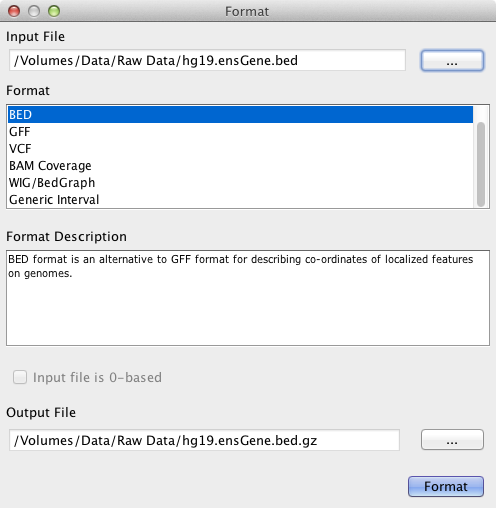
\includegraphics[type=png,ext=.png,read=.png,height=8cm]{images/FormatDialog}
\label{FormatDialog}
\caption{The Format Dialog}
\end{center}
\end{figure}

Components of the Format Dialog:

\begin{tabular}{l p{15cm}}
Input file & The text file to be formatted.\\
Format & The format of the input file.\\
Input is 1-based & Whether or not the input file's positional annotations start at 0 or 1.  In most cases, this is determined by the choice of Format.\\
Output file & The output file to be produced which can subsequently be loaded into Savant.\\
\end{tabular}

\subsection{Generating Coverage Files}
\label{GeneratingCoverageFiles}
In addition to formatting the file types described in Table~\ref{CompatibleFileFormatsTable}, the Format dialog is also used for generating coverage files.  These are used to display alignment data when the viewable range is too large to make individual reads discernible.  In such cases, Savant uses the coverage file to draw a continuous track indicating the level of read coverage across the viewable range.  Simply choose a .bam file as the input, and Savant will generate the corresponding .bam.cov.tdf file.  In order to serve as a coverage file, the .bam.cov.tdf file must be stored in the same location as the .bam file which it summarises.


\chapter{Navigation}

Navigation refers to changing the region of the genome which is being viewed by the browser. You can navigate either by interacting with the navigation toolbar (\S\ref{NavigationToolbar}) located at the top of the Savant main window, or by using the appropriate keyboard and mouse shortcuts (\S\ref{NavigationShortcuts}).

In Savant a location consists of two parts:  the current reference and the current visible range.  The current reference is typically a chromosome, so the term ``chromosome'' is used below, even though the reference in question could actually be any contiguous range of bases, and not necessarily a chromosome \textit{per se.}  The current range specifies a range of bases in the coordinate space of the current reference. 

\section{Navigation Toolbar}

\begin{figure}[h]
\label{NavigationToolbar}
\begin{center}
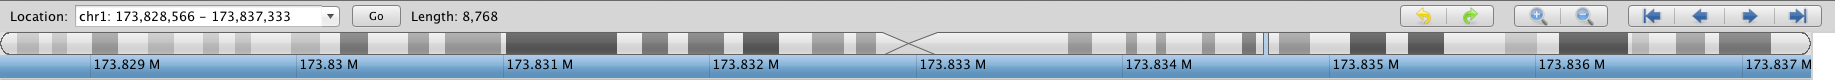
\includegraphics[type=png,ext=.png,read=.png,width=15cm]{images/NavigationBars}
\caption{Navigation Toolbar}
\end{center}
\end{figure}

The top row of the navigation toolbar contains the location field (\S\ref{LocationField}) and the navigation buttons (\S\ref{NavigationButtons}).  Below that are the genome bar and the ruler (\S\ref{GenomeBar}).

\subsection{Location Field}
\label{LocationField}
\begin{figure}[h]
\begin{center}

\includegraphics[type=png,ext=.png,read=.png]{images/LocationField}
\caption{Location Field}
\end{center}
\end{figure}

The location field displays the current visible range within the genome.  It can also be used to specify a new range in a number of ways, described in the table below.  Changes take effect by hitting {\sc return} or clicking the \textit{Go} button.

\begin{table}[h]
\begin{center}
\begin{tabular}{|l l l|}
\hline
1) & \multicolumn{2}{l|}{Clicking the downward-pointing triangle to reveal a menu of chromosomes.}\\
\hline
2) & \multicolumn{2}{p{15cm}|}{Type a gene name into the text field.}\\
& \multicolumn{2}{p{15cm}|}{Type a partial gene name and hit {\sc tab} to pop up a menu of matching genes.}\\
\hline
3) & \multicolumn{2}{l|}{Type a range specification into the text field:}\\
& &\\
& chr2:1000-2000 & chr2, range 1000-2000\\
& chr2 & chr2, range 1-1000\\
& 1000-2000 & in current chromosome, range 1000-2000\\
& 1000-900 & in current chromosome, range 900-1000 (equivalent to 900-1000)\\
& 1000+2000 & in current chromosome, range 1000-3000\\
& 1000 & in current chromosome, start position at 1000, keeping current range-length\\
& +1000 & 1000 bases to the right of the current start, keeping same range-length\\
& -1000 & 1000 bases to the left of the current range, keeping same range-length\\
\hline
\end{tabular}
\caption{Specifying Ranges Using the Location Field}
\end{center}
\end{table}

\subsection{Navigation Buttons}
\label{NavigationButtons}

\begin{figure}[h]
\begin{center}

\includegraphics[type=png,ext=.png,read=.png]{images/NavigationButtons}
\caption{Navigation Buttons}
\end{center}
\end{figure}
At the top right of the Navigation Toolbar are eight buttons which perform a variety of navigation-related tasks.  From left to right these are:  \textit{Undo, Redo, Zoom In, Zoom Out, Beginning, Pan Left, Pan Right,} and \textit{End.}

\textit{Undo} lets you undo your previous navigation action.  It can be used repeatedly to undo multiple navigation actions.  \textit{Redo} cancels the effect of the most recent \textit{Undo.}

\textit{Zoom In} and \textit{Zoom Out} change the visible range by a factor of two, keeping it centred on the same location.

\textit{Pan Left} and \textit{Pan Right} shift the visible location left or right by half the width of the screen.

\textit{Beginning} and \textit{End} allow you to navigate quickly to the beginning or end of the current chromosome.

\subsection{Genome Bar and Ruler}
\label{GenomeBar}

\begin{figure}[h]
\begin{center}
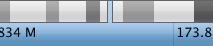
\includegraphics[type=png,ext=.png,read=.png]{images/RangeSelection}
\caption{Genome Bar and Ruler}
\end{center}
\end{figure}
Below the location field and the navigation buttons lies the genome bar.  This bar highlights in blue the current visible region in the context of the genome. If the current genome has associated cytoband information, it will be displayed in this bar.  You can select a new range by clicking and dragging within the bar.

Underneath the genome bar is the ruler, which indicates the current viewable range in the coordinate space of the current chromosome.

\section{Mouse and Keyboard Shortcuts}
\label{NavigationShortcuts}
Navigation can be done very quickly using a number of mouse and keyboard shortcuts described in the tables below.

\begin{table}[ht] 
\begin{center}
\begin{tabular}{|l l|}
\hline
Keys & Action \\
\hline                    
{\sc shift}+{\sc left} & pan left  \\
{\sc shift}+{\sc right} & pan right \\ 
{\sc shift}+{\sc home} & move to start of chromosome  \\
{\sc shift}+{\sc end} & move to end of chromosome \\ 
{\sc shift}+{\sc up} & zoom in \\
{\sc shift}+{\sc down} & zoom out \\  
\hline
\end{tabular}
\caption{Navigation Using the Keyboard}  
\end{center}
\end{table} 

In addition to these navigation shortcuts, there are a number of other useful shortcuts, described in Table~\ref{OtherShortcuts}
\begin{table}[h] 
\begin{center}
\begin{tabular}{|l l|}  
\hline                      
Keys & Action \\
\hline                    
Click and drag left/right & pan left/right  \\
{\sc ctrl/cmd} + scroll-wheel up/down & pan left/right  \\
{\sc ctrl/cmd} + Click and drag & zoom in on selected region  \\
{\sc shift} + Click and drag  & select all records in region  \\
\hline
{\sc ctrl/cmd + z} & undo range change  \\
{\sc ctrl/cmd + y} & redo range change \\ 
{\sc ctrl/cmd + i} & export track images (see \S\ref{ExportingImages}) \\ 
{\sc ctrl/cmd + b} & bookmark current location (see \S\ref{Bookmarks}) \\ 
{\sc ctrl/cmd + j} & crosshair (see \S\ref{HighlightingAreas}) \\ 
{\sc ctrl/cmd + k} & plumbline (see \S\ref{HighlightingAreas}) \\ 
{\sc ctrl/cmd + l} & spotlight (see \S\ref{HighlightingAreas}) \\ 
\hline
\end{tabular}
\caption{Other Shortcuts}  
\label{OtherShortcuts}
\end{center}
\end{table} 

\chapter{Visualisation Features}

In addition to making it easy to navigate quickly and efficiently through the genome, Savant provides a variety of mechanisms for making it easier to visualise the data more effectively.

\section{Track Locking}
\label{TrackLocking}
Individual tracks can also be locked to a particular range so that they are not updated until they are unlocked. Locked tracks can be used as overview profiles from which subregions can be selected to specify range changes for other tracks. To lock a track, select the \textit{Lock Track} option from the track's \textit{Tools} menu. While a track is locked, you may select a subrange from the track (by using the mouse zoom options, described previously) which will become the new range for other, unlocked tracks. To unlock a track, go to the track's menu and uncheck the \textit{Lock Track} option.

\section{Selecting Records}
In most cases, a track consists of a collection of underlying records, which can be selected individually.  By default, selected records are highlighted in green.  Selected records remain selected when the display mode changes, so  for instance you could select an arc in Read Pair (Arc) mode and then switch to Mismatch mode to see the details of the selected reads.  Records selected in a track are also selected in the Data Table (Chapter~\ref{DataTable}).

\section{Popup Menus}
Hovering the mouse over a track will pop up a menu which provides information about the record under the mouse, as shown in Figure~\ref{TrackPopup}.  The details of what fields are displayed in the popup is dependent on the type of data contained in the track.  To make it clearer exactly which record corresponds to the popup, the track will give the record a reddish tint while the popup is open.

At the bottom of the popup menu are a number of blue menu-items which allow you to perform specific actions on the current record.  The \textit{Select/Deselect} and \textit{Add to Bookmarks} items are common to popups for all track types; certain track types may add additional items as appropriate.

\begin{figure}[h]
\begin{center}
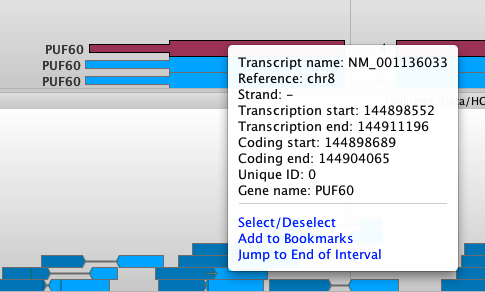
\includegraphics[type=png,ext=.png,read=.png,width=9cm]{images/TrackPopup}
\caption{Track Popup}
\label{TrackPopup}
\end{center}
\end{figure}

\section{Highlighting Areas of Interest}
\label{HighlightingAreas}

Often, it is helpful to focus one's attention on a particular portion of the display.  Savant provides three tools for making this easier, found under the \textit{View} menu.

The \textit{Crosshair} tool displays a crosshair cursor and shows the current track-space coordinates of the mouse.  This is intended to make it easier to identify particular features by location.  Note that the current location (without the crosshair) is also shown in the lower left of the Savant window. 

The \textit{Plumbline} tool displays vertical bars which run across all the tracks, allowing you to clearly see how features on different tracks are aligned.

The \textit{Spotlight} tool is similar to the Plumbline tool, except that portions of tracks outside the spotlight area are dimmed to deemphasise them.

\chapter{Docking Framework}
\label{DockingFramework}

Savant features a docking framework which allows you to rearrange modules to your liking. Such modules include tracks and built-in items (e.g. Bookmarks, Variants, etc.) and plugins. Non-track modules are constrained to be docked to the sides of the UI and not among tracks. Similarly, track modules are constrained so that they cannot be docked among other modules.

While a number of important functions are presented here, the best way to learn all the features of the docking framework is to try using it.

\begin{figure}
\begin{center}
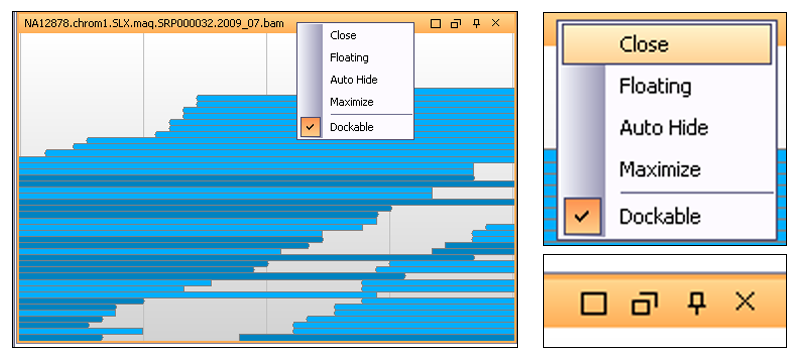
\includegraphics[type=png,ext=.png,read=.png,width=12cm]{images/dockingcontrols}
\caption[Docking Controls]{Left: A track module. Upper-right: Docking menu presented when the title bar of a module is right-clicked. Bottom-right: Docking controls embedded in the title bar of the module. The latter controls are {\it not} available in the Mac version.}
\end{center}
\end{figure}

\section{Showing and Hiding Modules}

By default, built-in modules are hidden. Hidden modules appear as tabs located on the region of the UI to which they are docked. A module is shown once the tab is clicked. Click the tab again to hide the module.

\begin{figure}
\begin{center}
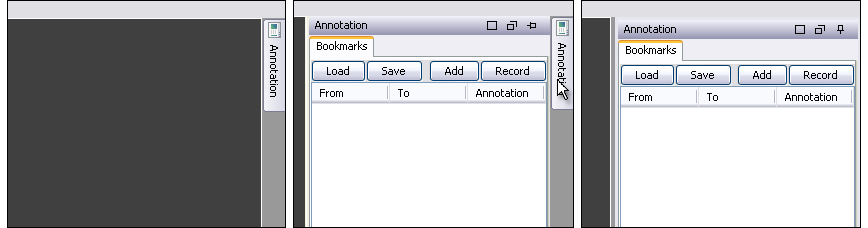
\includegraphics[type=png,ext=.png,read=.png,width=14cm]{images/hideshowmodules}
\caption[Hiding and Showing Modules]{Hiding and Showing Modules. Left: The Annotation module, hidden on the right of the Savant UI. Middle: The Annotation module, shown by clicking the Annotation tab. Right: The Annotation module, pinned so that it will remain shown even when you are interacting with other components of the UI. }
\label{HideShowModules}
\end{center}
\end{figure}

\section{Resizing Modules}

Modules can be resized. To resize a module, click an edge and drag it until it occupies the desired size. 

\section{Rearranging Modules}

Modules can be arranged in virtually any configuration within the UI. To move a module, click its title bar and drag it to the desired new location. While dragging, a grey outline will appear showing the location the module will occupy if the mouse is released. Track modules can be docked to the top or bottom of the track space, while other modules can be docked to any edge of the UI. In addition, modules can be docked on top of each other (in which case tabs will appear allowing one to switch between modules) or beside each other.

\begin{figure}
\begin{center}
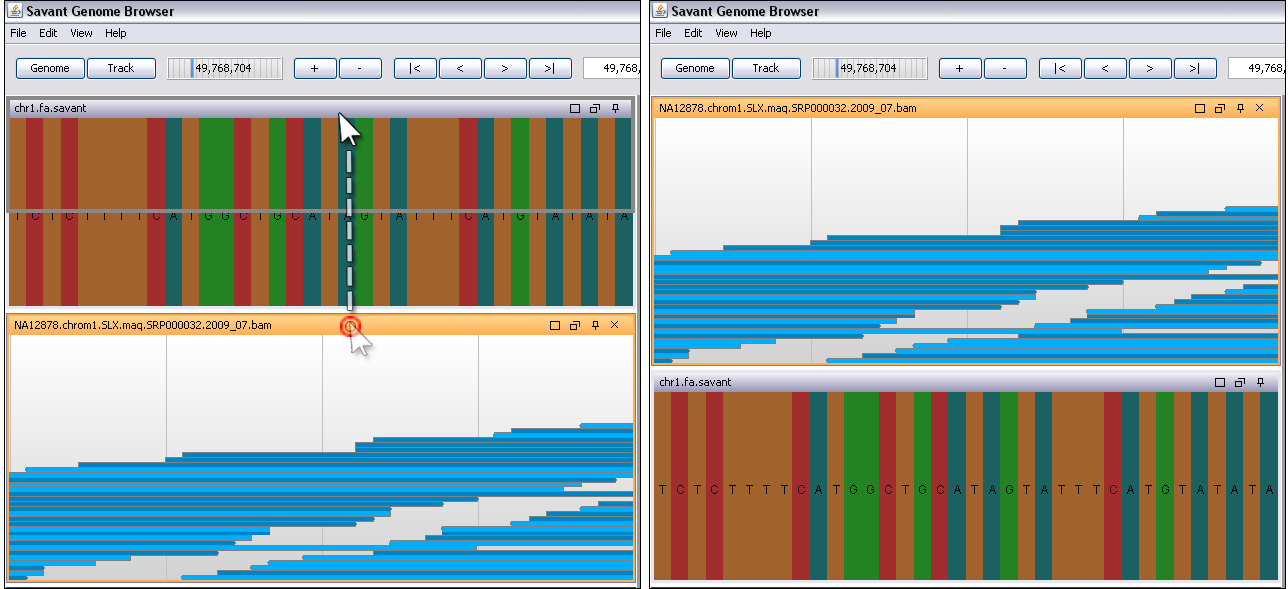
\includegraphics[type=png,ext=.png,read=.png,width=14cm]{images/arrangemodules}
\caption[Rearranging Modules]{Rearranging Modules. Left: Demonstration of the rearrangement process. Right: The result of the rearrangement.  }
\label{ArrangeModules}
\end{center}
\end{figure}

\section{Maximising and Restoring Modules}

A module can be maximised to occupy the entire screen or UI, to make interaction or visualisation with it easier, and then restored back to its original state among other modules to resume a concerted view. To maximise, press the embedded icon which resembles a square. To restore, press the embedded icon which resembles two overlapping squares (in the same location as the icon pressed to maximise). On a Mac, you can maximise and restore by double-clicking the title bar. The same functionality is possible through the title bar on Windows and Linux.

\section{Detaching and Attaching from and to the UI}

A module can be detached from the UI and moved to a separate location on the screen. This is particularly useful for multi-display setups where, for example, analytics modules can be moved to one display and tracks kept on another. To detach a module, press the embedded icon which resembles to squares. The detached module can then be moved to another location by clicking and dragging its title bar. To reattach it to the UI, press the embedded icon which resembles a square with an L-shape in it (in the same location as the icon pressed to detach it). On a Mac, you can detach and reattach by right-clicking the title bar and checking or unchecking Floating, respectively. The same functionality is possible through the title bar on Windows and Linux.


\chapter{Bookmarks}
\label{Bookmarks}
The Bookmarks module helps to keep track of interesting regions or to make annotations. At any time, you may add, remove, or seek to a bookmarked region by using buttons within the module or by using keyboard shortcuts. 

\begin{figure}
\begin{center}
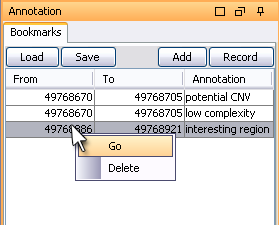
\includegraphics[type=png,ext=.png,read=.png,width=6cm]{images/bookmarks}
\caption{Bookmarks Module}
\end{center}
\end{figure}

\section{Adding and Removing Bookmarks}

A bookmark can be added by pressing the Add button ($\vcenter{\hbox{
\includegraphics{images/bkm_add.png}}}$) in the Bookmarks module's toolbar. The current range will be used for the bookmark, although the from and to coordinates of the bookmark can be adjusted by double clicking and changing them. The keyboard shortcut {\sc ctrl+b} (or {\sc cmd+b} on a Mac) can be used to quickly add a bookmark.

For tracks which contain multiple features (e.g. gene tracks), the track's \textit{Tools} menu provides a way to automatically create a bookmark for each of a track's features.

Bookmarks can be removed by selecting them and choosing the Delete button ($\vcenter{\hbox{
\includegraphics{images/bkm_rm.png}}}$).

\section{Seeking to a Bookmark}

A bookmark can be sought to by selecting it and choosing the Go option.

\section{Adding Annotations to Bookmarks}

An annotation can be added to a bookmark by double-clicking the Annotation field and typing in some text. 

\section{Saving and Loading Bookmarks}

As bookmarks are created, they are automatically stored as part of the current project file, and will be saved whenever the project is saved.

Bookmarks can be exported, to be reused in other sessions or to be shared with colleagues. To save the existing bookmarks, click the Save button ($\vcenter{\hbox{
\includegraphics{images/save2.png}}}$) in the Bookmarks module's toolbar. These bookmarks can subsequently be loaded by clicking the Load button ($\vcenter{\hbox{
\includegraphics{images/open.png}}}$).

Exported bookmarks are stored as a simple tab-delimited text file with four columns:  chromosome, start, end, and annotation.  Consequently, if you create your own tab-delimited file with this layout, it can be loaded into a Savant project as a set of bookmarks.

You can opt to append the loaded bookmarks to the existing bookmarks, or to replace the existing bookmarks entirely with the loaded ones.

Savant also gives you the option of adding padding to bookmarks to make them more prominent.  For instance, if you have loaded bookmarks from a text file containing SNP coordinates, you might want to add padding so that navigating to a SNP will display it centred in the display area; without padding, selecting one of these SNP bookmarks would set the range so that the selected SNP filled the entire display.

\chapter{Data Table}
\label{DataTable}

The Data Table is a plugin (see Chapter~\ref{Plugins}) which is installed by default as part of Savant.  The Data Table module displays the data in the current range in a tabular format, with the records being rows and the fields being columns.

The data is automatically updated when the range in the main track display changes, unless the \textit{Auto Update} checkbox is unchecked.  The \textit{Show Only Selected} checkbox allows you to filter the table, showing only records which are selected in the current track.

Double-clicking on a row in the data table will select the corresponding record in the track display.

\begin{figure}[h]
\begin{center}
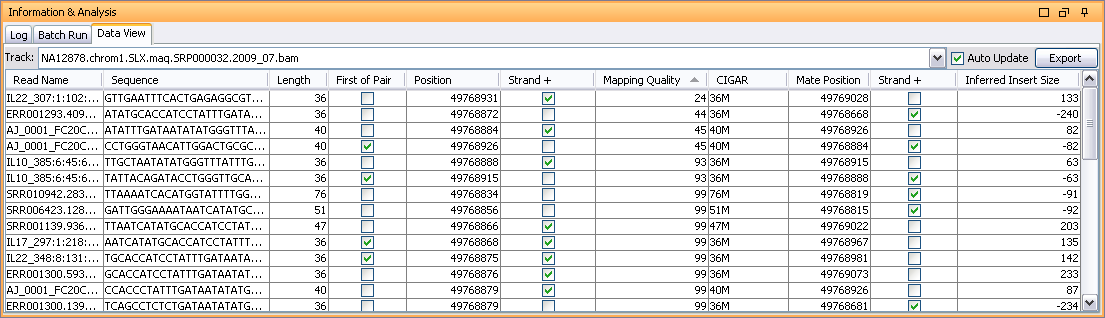
\includegraphics[type=png,ext=.png,read=.png,width=16cm]{images/tableview}
\caption[Data Table Module]{Data Table Module, showing data from a read alignment track.}
\end{center}
\end{figure}

\section{Changing Tracks}

The Data Table only displays data from a single track at a time. To change the track whose data is being displayed, a drop-down list of tracks is provided from which to choose.

\section{Sorting Rows}

The entries in the Data Table can be sorted by clicking the field header by which the rows are to be sorted.  Subsequent clicks on the field header toggle between sorting in ascending order and descending order.

\section{Exporting Data}

The data being viewed in the Data Table can be exported to a text file by clicking the Export button.

The format of the resulting text file depends on the type of the track being exported.  Sequence tracks are exported as Fasta files.  BAM alignment tracks are exported as SAM files.  All other track types are simply exported as tab-delimited text.

\chapter{Plugins}
\label{Plugins}

Savant is able to integrate plugins, allowing for powerful extensions of the browser. To learn how to develop a plugin, see the {\bf Developer's Guide} downloadable from the Savant web-site.

\section{Installing and Uninstalling Plugins}
\label{InstallingPlugins}

To install a plugin, choose \textit{Plugin Manager\ldots} from the \textit{Plugins} menu.  Savant will present the dialog shown in Figure~\ref{PluginManager}.  This dialog lists all the plugins which are currently installed.  Selecting one of plugins from the list will display information about the plugin's version and status, and provide a button to allow uninstalling the plugin.

\begin{figure}[h]
\begin{center}
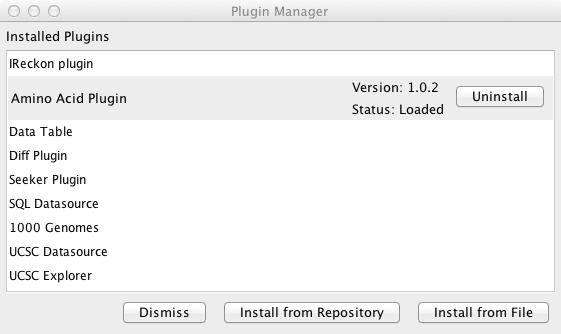
\includegraphics[type=png,ext=.png,read=.png,width=15cm]{images/PluginManager}
\caption{Plugin Manager Dialog}
\label{PluginManager}
\end{center}
\end{figure}

Clicking \textit{Install from Repository} will bring up a second dialog (Figure~\ref{PluginRepository}) which lets you browse the plugins available on the Savant web-site.  Plugins in the repository are segregated by Savant version, since Savant 2.0.0 is not compatible with plugins developed for older versions of Savant.

Third-party plugins which are not available through the Savant Plugin Repository can be installed using the \textit{Install from File} command, which lets you select a JAR file to be installed.  \textit{Install from File} will copy the selected file into Savant's plugin directory and make it available to Savant.

Some third-party plugins may require ancillary files (e.g. supporting libraries or data files).  Installing this sort of plugin cannot be done through the Plugin Manager dialog; in such cases the necessary files must be manually copied into the \textit{.savant/plugins} directory (\textit{savant\textbackslash plugins} on Windows).

\begin{figure}[h]
\begin{center}
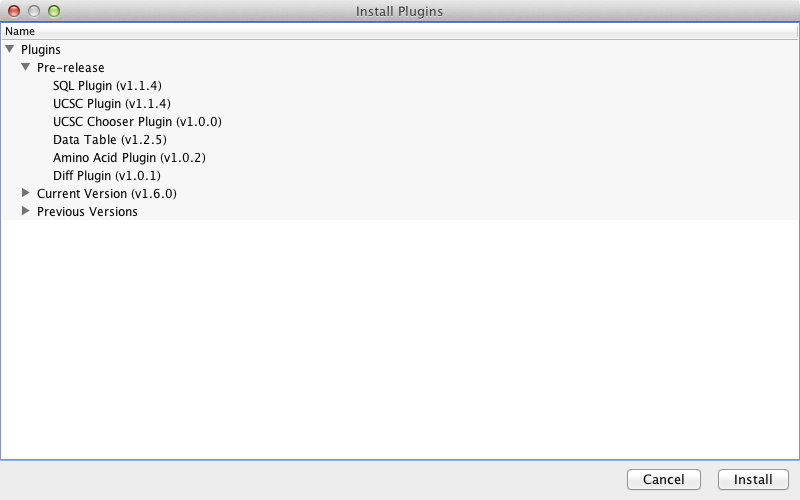
\includegraphics[type=png,ext=.png,read=.png,width=15cm]{images/PluginRepository}
\caption{Plugin Repository Dialog}
\label{PluginRepository}
\end{center}
\end{figure}

\section{Using Plugins}

Every plugin works differently and may or may not have a user interface. For instructions on how to use a third-party plugin, see the developer's documentation.  Savant supports three general types of plugins, which are described below.

\subsection{Panel Plugins}
Typical plugins (such as the built-in Data Table and UCSC Explorer plugins) are presented in tabs at the bottom left of the Savant user interface.  Click the tab to reveal the plugin's user interface.  The windows for these plugins can be detached, docked and rearranged, as described in Chapter~\ref{DockingFramework}.

Plugins can be temporarily disabled by unchecking the corresponding menu-item on the \textit{Plugins} menu.  This is a less extreme measure than uninstalling the plugin; a disabled plugin is still installed and can easily be reenabled by reselecting its menu-item from the \textit{Plugins} menu.

\subsection{Tool Plugins}
New in Savant 2.0 are ``tool plugins'', which provide a way to integrate external applications into Savant.  To the end-user, these are functionally similar to panel plugins, but where panel plugins consist of Java code packaged inside a JAR file, tool plugins consist of an XML file providing instructions on how to invoke an external application.  The format of this XML file is described in the Developer Manual.

Like panel plugins, tool plugins present their user interface in a dockable tab at the bottom left of the Savant user interface, and can be enabled/disabled from the \textit{Plugins} menu.

The GATK and SRMA plugins are examples of tool plugins.

\subsection{Data Source Plugins}
Data source plugins are a special class of plugins which extend Savant, allowing it to access data in non-standard ways.  Data source plugins do not have a tab at the bottom left of the Savant window, but instead are accessed through the \textit{Load Track from Other Datasource} menu-item.\footnote{Or in the case of genomes, from the \textit{Other Datasource} button on the genome dialog.}

The UCSC and SQL plugins are both examples of data source plugins.

\chapter{Other Features}

\section{Exporting Images}
\label{ExportingImages}
Track images from Savant can be exported as PNG files using the \textit{File~\textgreater~Export~Images} command.  This command brings up a dialog which allows you to select the tracks you want to appear in the output.  By default, none of the tracks are selected, and you use the arrow buttons to move them from the unselected (left) side to the selected (right) side of the dialog.

Checking the \textit{Always select all} check-box means that the next time the dialog is displayed, all tracks will start on the selected side of the dialog.

Optionally, you may enter a single base which will be highlighted in the output PNG file using a plumbline (as described in \S\ref{HighlightingAreas}).

\begin{figure}[h]
\begin{center}
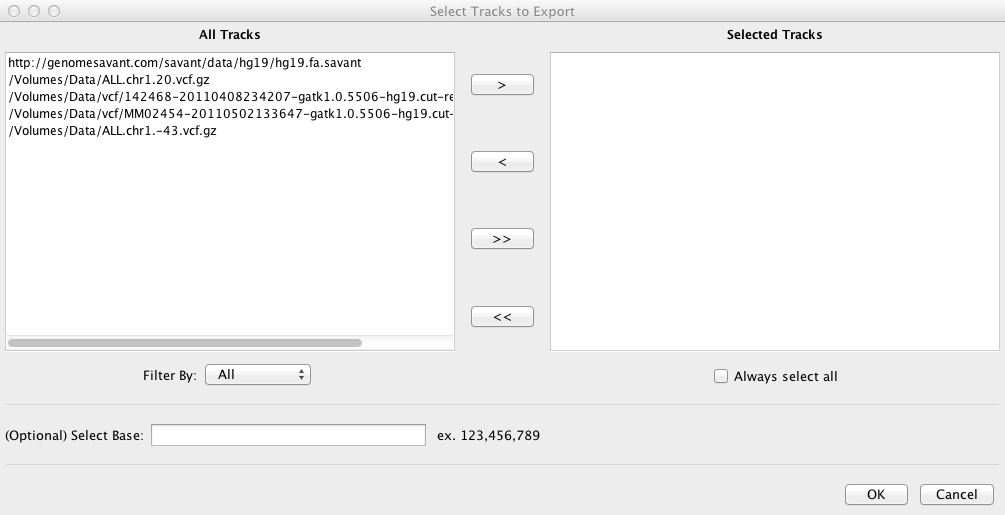
\includegraphics[type=png,ext=.png,read=.png,width=15cm]{images/ExportImage}
\caption{Export Image Dialog}
\end{center}
\end{figure}

\chapter{Variants}
\label{Variants}
Savant 2 provides improved support for viewing variant data in VCF files.  In addition to being able to open Tabix-formatted VCF files as variant tracks, Savant 2 also provides a Variation tab at the right of the user interface (next to the Bookmarks tab).  This tab provides a variety of ways of exploring variation data, as described in \S\ref{VariationTab}.

\section{Variant Tracks}
\label{VariantTracks}
Variant data can be loaded into Savant using the \textit{Load Track from XXX\ldots} commands.  Loading a VCF file in this fashion will create a new track in the main display area.  As with other data types, the VCF file must first be formatted and indexed as a Tabix file in order to be usable (see \S\ref{UsingFormatDialog}).

SNPs are displayed with a vertical line in the colour of the alternate (non-reference) base.  Participants drawn from the VCF file are arranged vertically.  A gap in the vertical line indicates that a particular participant lacks that variant.  If a variant is heterozygous for a participant, that portion of the line will be drawn using a paler version of the associated colour.

Insertions and deletions are displayed in the same manner as SNPs, with a single vertical line (black for deletions, magenta for insertions).  The variant track makes no attempt to visually indicate the extent of the inserted or deleted material.  In order to see what was actually substituted by the indel, you will need to hover the mouse over the variant track, and the popup will provide the details of the substitution that took place.

\section{Variation Module}
\label{VariationTab}

The Variation module groups together four different ways of viewing aggregated variant data.  While variant tracks contain data only from a single VCF file, the visualisations on the Variation module comprise data from all currently-open variant tracks.

The variation module maintains its own visible range, which is distinct from the visible range for the main track display area.  Changing the range in the variation module has no effect on the main range.  The reverse is not true, since if you move the main display range outside the variation module's range (e.g. by shifting to another chromosome), the variation module will update its range to ``follow'' your navigation.

At the top of the variation module is a field for entering the module's desired visible range.  The variation module also has its own Zoom In and Zoom Out buttons to alter its visible range.

At the top right of the variation module is the \textit{Controls} button.  This is used to select which participants in a dataset are considered to be controls (as opposed to cases).  When graphing allele frequency, the control and case participants are graphed separately.

\subsection{Variation Table}

The variation table provides a spreadsheet-like summary of all variants in the variation module's current display range.  Double clicking on  row will centre the main track display on the position of that variant.

\subsection{Variation Map}

The variation map provides a graphical overview of all variants in the variation module's display range.  Variant records are arranged vertically by position, but the scale is non-linear since the gaps between variants are squeezed down.  Participants are laid out horizontally, using the same colour scheme as described for variant tracks (\S\ref{VariantTracks})

\subsection{Allele Frequency Plot}

The allele frequency plot graphs frequencies of each allele for each variant location.  Like the variation map, the allele frequency display is arranged vertically by position, with a non-linear scale.

If controls have been specified, allele frequencies for controls will be displayed on the left of the central axis, while case allele frequencies will be displayed to the right of the central axis.

\subsection{Linkage Disequilibrium Plot}

The linkage disequilibrium plot graphs LD values calculated using D$^\prime$ or r$^2$.  Variant locations are used as the loci for the LD calculation (i.e. there is no attempt to segregate ranges into groups).

\chapter{Preferences}
\label{Preferences}

The preferences dialog allows you to configure a number of Savant features.  The dialog is invoked by the \textit{Preferences} menu-item, which is found under the Savant application menu on Mac and under the \textit{Edit} menu on Windows and Linux.  Preferences are divided into five categories:  \textit{Colour Schemes, General Settings, Interface Settings, Remote Files,} and \textit{Track Resolutions}.  Each category appears on a separate panel in the preferences dialog.

As described in Appendix~\ref{SavantHomeDirectory}, these settings are stored in the \textit{savant.settings} file in your Savant home directory.  Deleting the \textit{savant.settings} file will restore Savant to its factory defaults.

\section{Colour Settings}
\textit{Colour Settings} allow you to adjust the colours which are used for rendering the various track types.

\section{General Settings}
\textit{General Settings} controls some behaviours of the Savant application.  At present, all of these happen to involve connecting to the savantbrowser.com web-site at startup time.

By default, Savant contacts the savantbrowser.com web-site at startup time, to determine whether a newer version of Savant has been released.  Unchecking the \textit{Check version on startup} to disable this feature if you do not wish to be reminded of new versions.

At startup, Savant also contacts savantbrowser.com to retrieve the Savant news feed.  Uncheck the \textit{Show Start Page} check-box to disable this behaviour; at startup Savant will display a blank page instead of the news page.

As an aid to our developers, as part of its startup process Savant reports back to the savantbrowser.com web-site with information about the usage environment.  The information reported is summarised in Table~\ref{AnonymousData}.  If you wish to disable this feature, un-check the \textit{Collect anonymous statistics about usage} check-box.

\begin{table}[h]
\begin{center}
\begin{tabular}{|l l|}
\hline
Information & Example\\
\hline\hline
time & 2012/02/16 14:18:58\\
language & English\\
time zone & America/Toronto\\
Savant version & 2.0.0\\
Savant build & beta\\ 
IP address & 128.100.3.60\\
Java version & 1.6.0\_23\\
Java vendor & Sun Microsystems Inc.\\
operating system & Linux\\
OS version & 3.0.0-15-generic\\
architecture & amd64\\
region & CA\\
\hline
\end{tabular}
\caption{Anonymous Usage Stats}
\label{AnonymousData}
\end{center}
\end{table}

\section{Interface Settings}
This section allows you to set the default heights for various BAM,and interval tracks.

In addition, you can enable or disable the display of popup menus and legends on tracks.

\section{Remote Files}
The \textit{Remote Files} section allows you to configure Savant's access and caching of remote files.  Any changes to settings on this panel will not take effect until the next time Savant is launched.

Un-checking the \textit{Enable remote file caching} button will disable the caching of remote files completely.  This is not recommended, because without caching, performance will be terrible.

By default, cache files are kept in the \textit{cache} subdirectory of your Savant home directory.  You can move it to another location if your home directory is located on a file-system where space is at a premium.

Remote file caching uses a default block size of 64kB.  There probably is no good reason to change this.

The cache directory can grow to consume a considerable amount of disk space.  If you wish to free up some disk space, you can use the \textit{Clear remote file cache} button.

\section{Track Resolutions}

This selection allows you to set a range threshold for each track type, above which the track will not attempt to render data.  When the display range is above a track's threshold, the track will display either a ``Zoom in to see data'' message or a coverage track (if available).

\appendix
\chapter{Savant Home Directory}
\label{SavantHomeDirectory}

By default, Savant stores settings, plugins, and temporary files in your home directory in a folder called \textit{.savant} on Mac and Linux, or \textit{savant} on Windows.  In most cases, it should not be necessary to delve into this directory, but it can be useful to know what is stored there.  Table~\ref{SavantDirectory} summarises the contents of the \textit{.savant} directory.

\begin{table}[h]
\begin{tabular}{|l p{12cm}|}
\hline
cache & Keeps a cache of files accessed from remote URLs.  Over time, this directory may use up a considerable amount of disk space. It can be cleared using the \textit{Clear remote file cache} option in the \textit{Preferences} dialog (Chapter~\ref{Preferences}).\\
index & Stores index files for remote BAM, Tabix, and Fasta files.\\
plugins & The Plugin Manager dialog (\S\ref{InstallingPlugins}) installs plugins in this directory.\\
projects & Default location for Savant project (\textit{.svp}) files.\\
savant.settings & Stores values for Savant preferences.  Edit this file at your own risk.\\
\hline
\end{tabular}
\caption{Contents of \textit{.savant} Directory}
\label{SavantDirectory}
\end{table}

\end{document}
